\documentclass[a4paper]{article}

\usepackage[utf8x]{inputenc}    
\usepackage[T1]{fontenc}
\usepackage{tikz}

\usepackage[francais,bloc,completemulti]{automultiplechoice}    
\begin{document}

\setdefaultgroupmode{withoutreplacement}

\element{general}{
  
  \begin{question}{carre-a}
    \QuestionIndicative
    Choisissez le nombre que vous voulez
    \begin{reponseshoriz}[o]
      \mauvaise{2}\scoring{2,setglobal.Nombre=2}
      \mauvaise{3}\scoring{3,setglobal.Nombre=3}
      \mauvaise{4}\scoring{4,setglobal.Nombre=4}
      \mauvaise{5}\scoring{5,setglobal.Nombre=5}
    \end{reponseshoriz}
  \end{question}
  
  \begin{questionmultx}{carre-b}
    \AMCdontAnnotate\bareme{MAX=2}
    Quel est son carré ?
    \AMCnumericChoices{}{digits=2,approx=1,alsocorrect=Nombre**2}
  \end{questionmultx}
}

\element{general}{

  \begin{minipage}{.3\linewidth}
    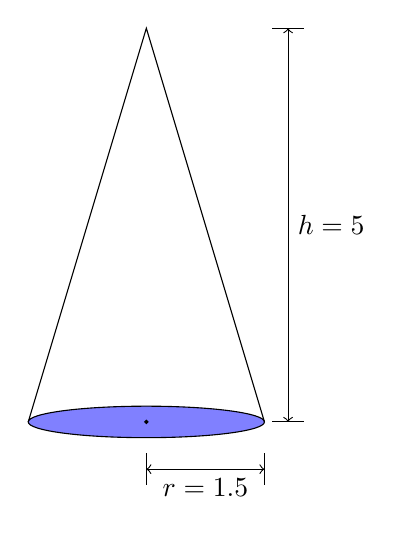
\begin{tikzpicture}
      \draw[fill=blue!50] (0,0) ellipse (1.5 and 0.2);
      \draw (1.5,0) -- (0,5) -- (-1.5,0);
      \draw (1.6,0) -- (2,0);
      \draw (1.6,5) -- (2,5);
      \draw[<->] (1.8,0) -- (1.8,5);
      \node[right] at (1.8,2.5) {$h=5$};
      \draw (0,-0.4) -- (0,-0.8);
      \draw (1.5,-0.4) -- (1.5,-0.8);
      \draw[<->] (0,-0.6) -- (1.5,-0.6);
      \node[below] at (0.75,-0.6) {$r=1.5$};
      \draw[fill=black] (0,0) circle (0.02);
    \end{tikzpicture}
  \end{minipage}
  \begin{minipage}{.65\linewidth}
    \begin{questionmultx}{cone-a}
      Quelle est la surface du disque bleu ?
      \AMCnumericChoices{pi*1.5^2}{digits=3,decimals=2,exponent=2,approx=2,sign=false,exposign=true,expovertical=true,keepas=Surface}
    \end{questionmultx}
    
    
    \begin{questionmultx}{cone-b}
      Quel est le volume du cône ?
      \AMCnumericChoices{pi*1.5^2*5/3}{digits=3,decimals=2,exponent=2,approx=2,sign=false,exposign=true,expovertical=true,alsocorrect=Surface*5/3}
    \end{questionmultx}
  \end{minipage}
  
}

\element{general}{
  \begin{questionmultx}{pipi2-a}
    Combien vaut $\pi$ ?
    \AMCnumericChoices{pi}{digits=3,decimals=2,sign=false,keepas=Pi}
  \end{questionmultx}

  \begin{questionmultx}{pipi2-b}
    Combien vaut $\pi^2$ ?
    \AMCnumericChoices{pi^2}{digits=3,decimals=2,sign=false,approx=1,alsocorrect=Pi**2}
  \end{questionmultx}
}

\element{general}{
  \begin{questionmultx}{circonf}
    Quelle est la circonférence d'un cercle de rayon $r=2$ ?
    \AMCnumericChoices{2*2*pi}{digits=3,decimals=1,approx=1,sign=false}
  \end{questionmultx}
}

\exemplaire{10}{    

%%% debut de l'en-tête des copies :    

\noindent{\bf QCM  \hfill TEST}

\vspace*{.5cm}
\begin{minipage}{.4\linewidth}
\centering\large\bf Test\\ Examen du 01/01/2008\end{minipage}
\champnom{\fbox{    
                \begin{minipage}{.5\linewidth}
                  Nom et prénom :

                  \vspace*{.5cm}\dotfill
                  \vspace*{1mm}
                \end{minipage}
         }}
\vspace{2ex}
       
%%% fin de l'en-tête

\restituegroupe{general}

}   

\end{document}
